%!TEX root = /Users/dylanmorano/Documents/School/Senior/Senior Design/semester-one-report/latexmain/reportone.tex

\section{Free Hanging Resonance Tests with PMNT Piezoelectric Sensor}

Several experiments were carried out on a 20 foot long, 1/4th inch 114R steel rod. These tests were performed in order to determine the methodology for finding resonant frequencies of the rod when excited with both longitudinal (axial) and transverse (shear) waves. The purpose of these tests was also to experimentally validate the described method for determining resonant frequencies in a free hanging metal rod. Tests were performed using multiple types of piezoelectric sensors as contact microphones for observing and analyzing the response of exciting vibrations along the rod. 

\subsection{Experimental Procedure}

A steel rod was suspended from 4 equally spaced laboratory stools using elastic bands in order to isolate the vibrations from the rod to the stools. This method was used in order to attempt to represent an ideal free hanging rod with no support on either end. A PMNT piezoelectric sheet was attached around the rod at one of the free hanging ends and connected to a computer’s sound card using a 3.5mm patch cable. The attached piezoelectric sensor and rod can be seen below in Figure~\ref{fig:PMNT_rod} as well as the elastic suspension of the rod in Figure~\ref{fig:rubbleband}.

\begin{figure}[h]
\centering
\begin{minipage}{.5\textwidth}
  \centering
  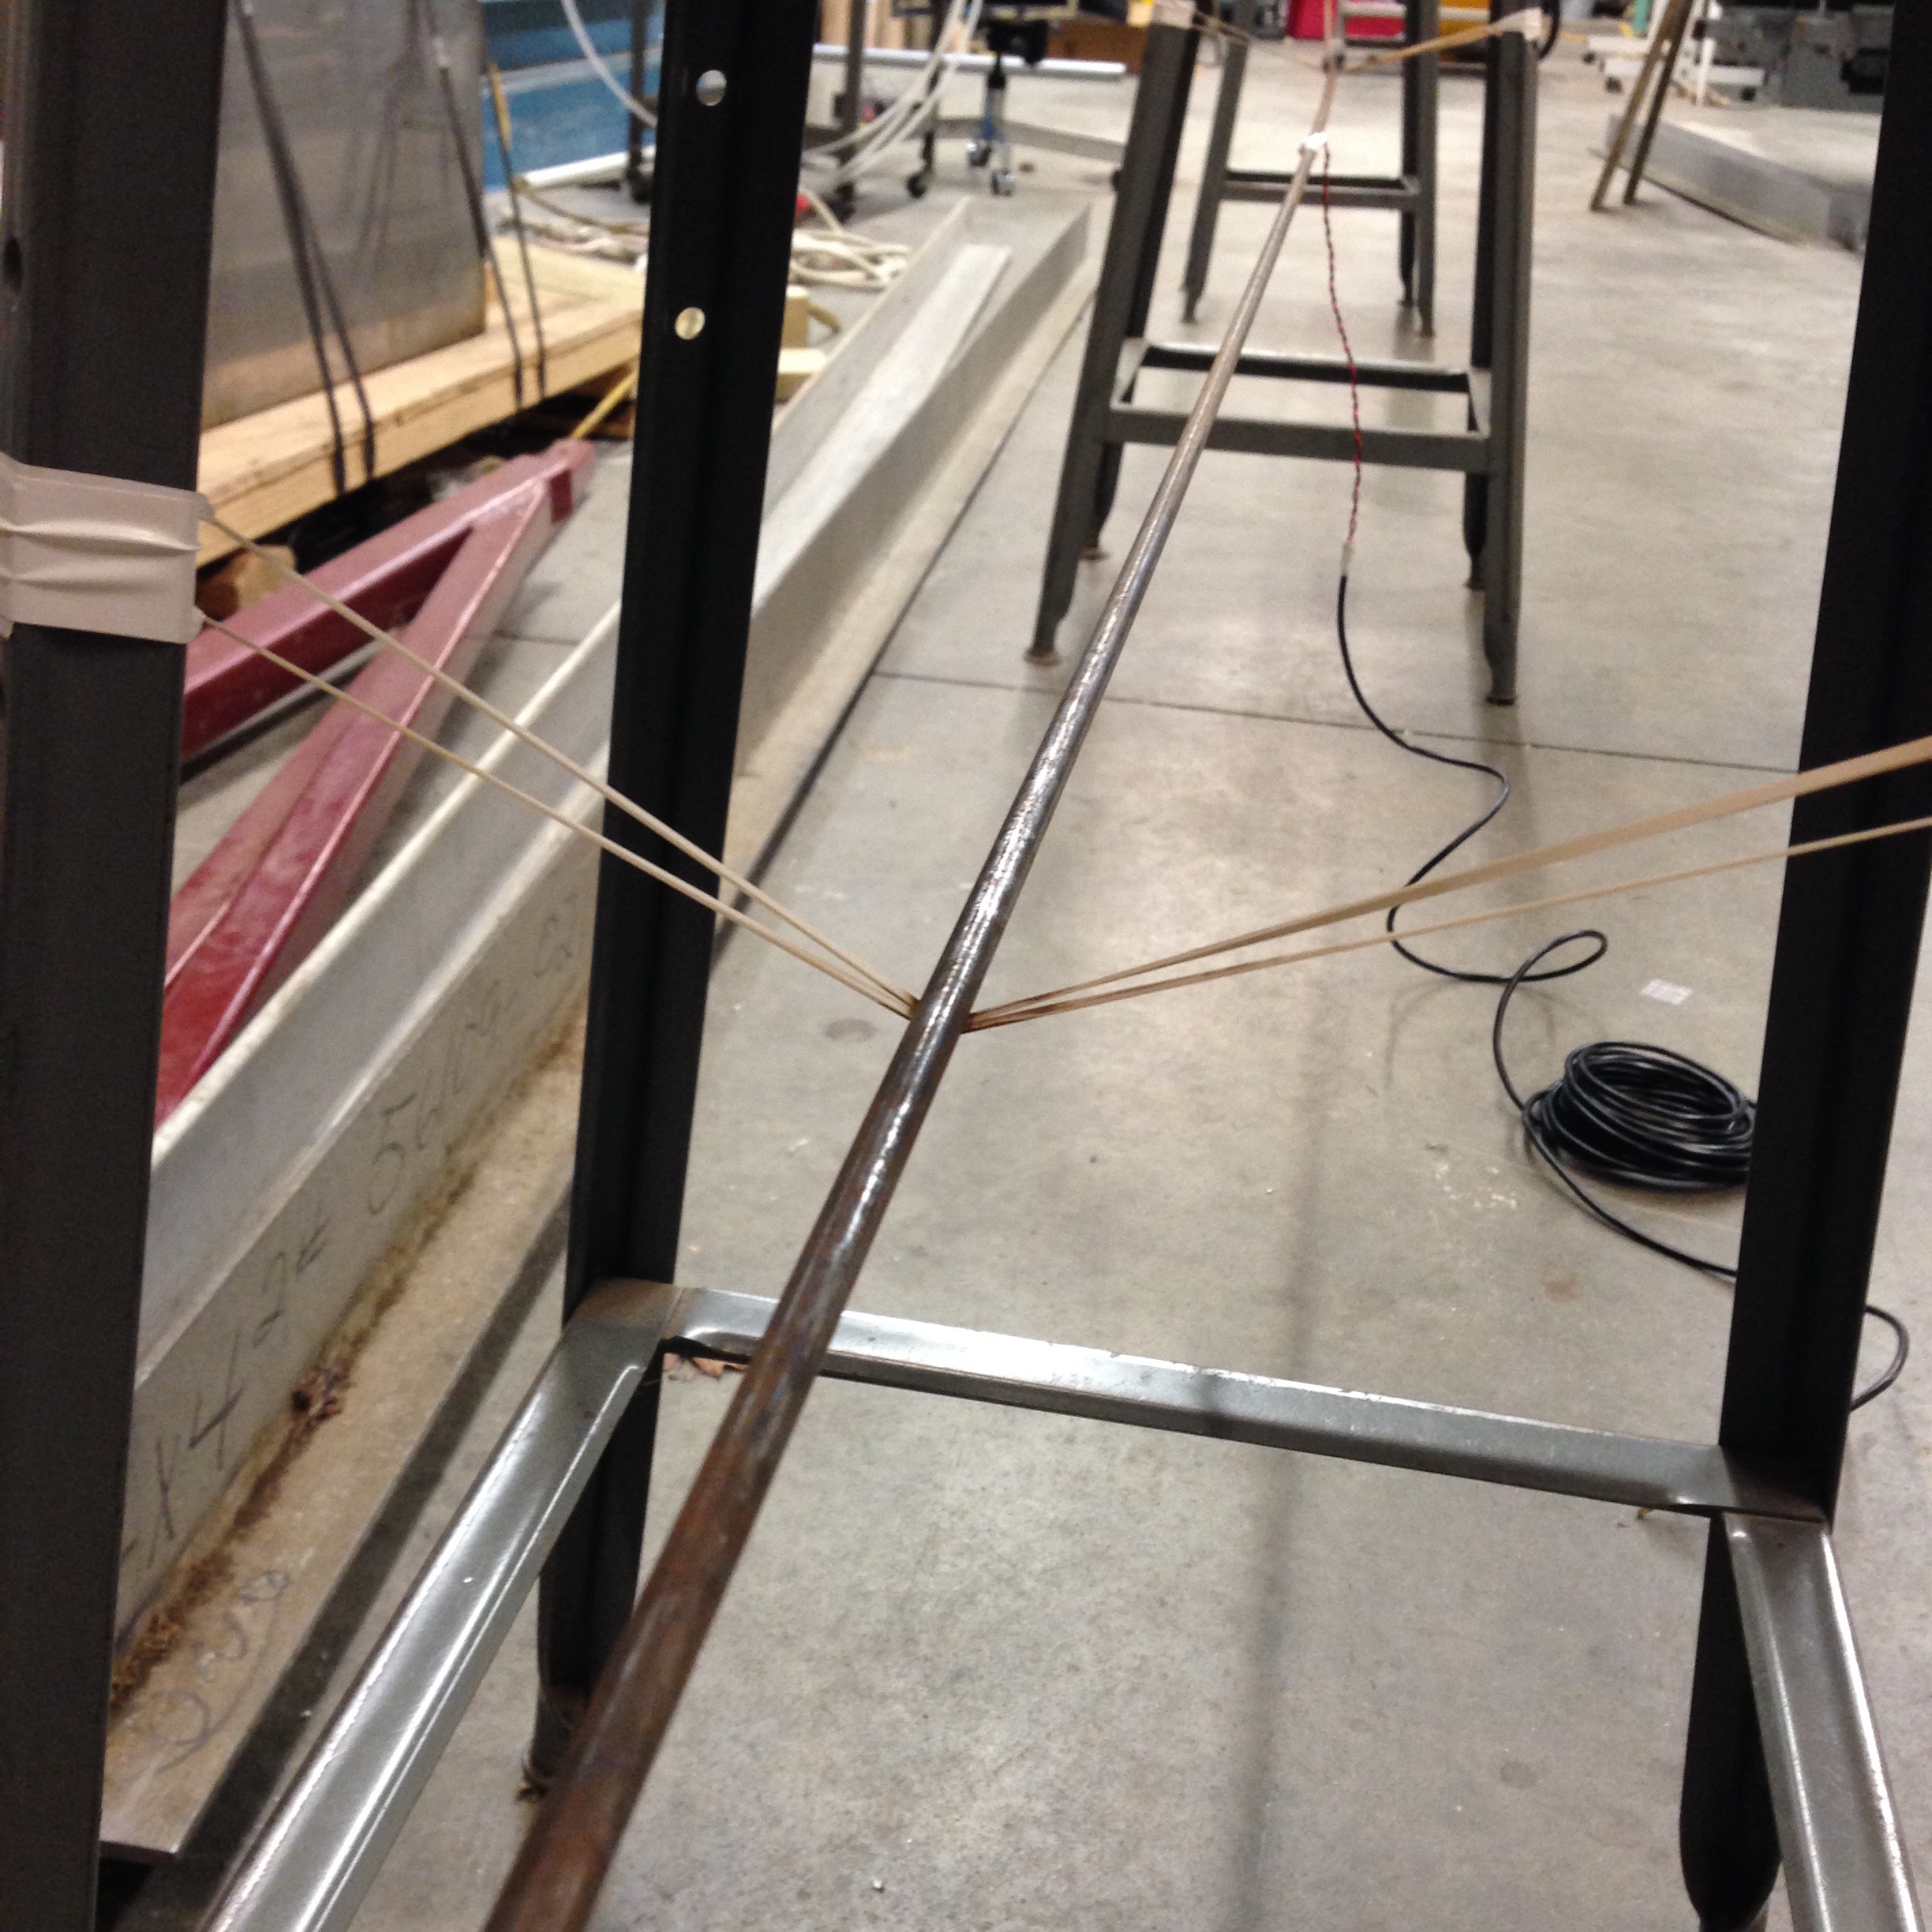
\includegraphics[width=.95\linewidth]{../figures/bands.jpg}
  \captionof{figure}{A figure}
  \label{fig:PMNT_rod}
\end{minipage}%
\begin{minipage}{.5\textwidth}
  \centering
  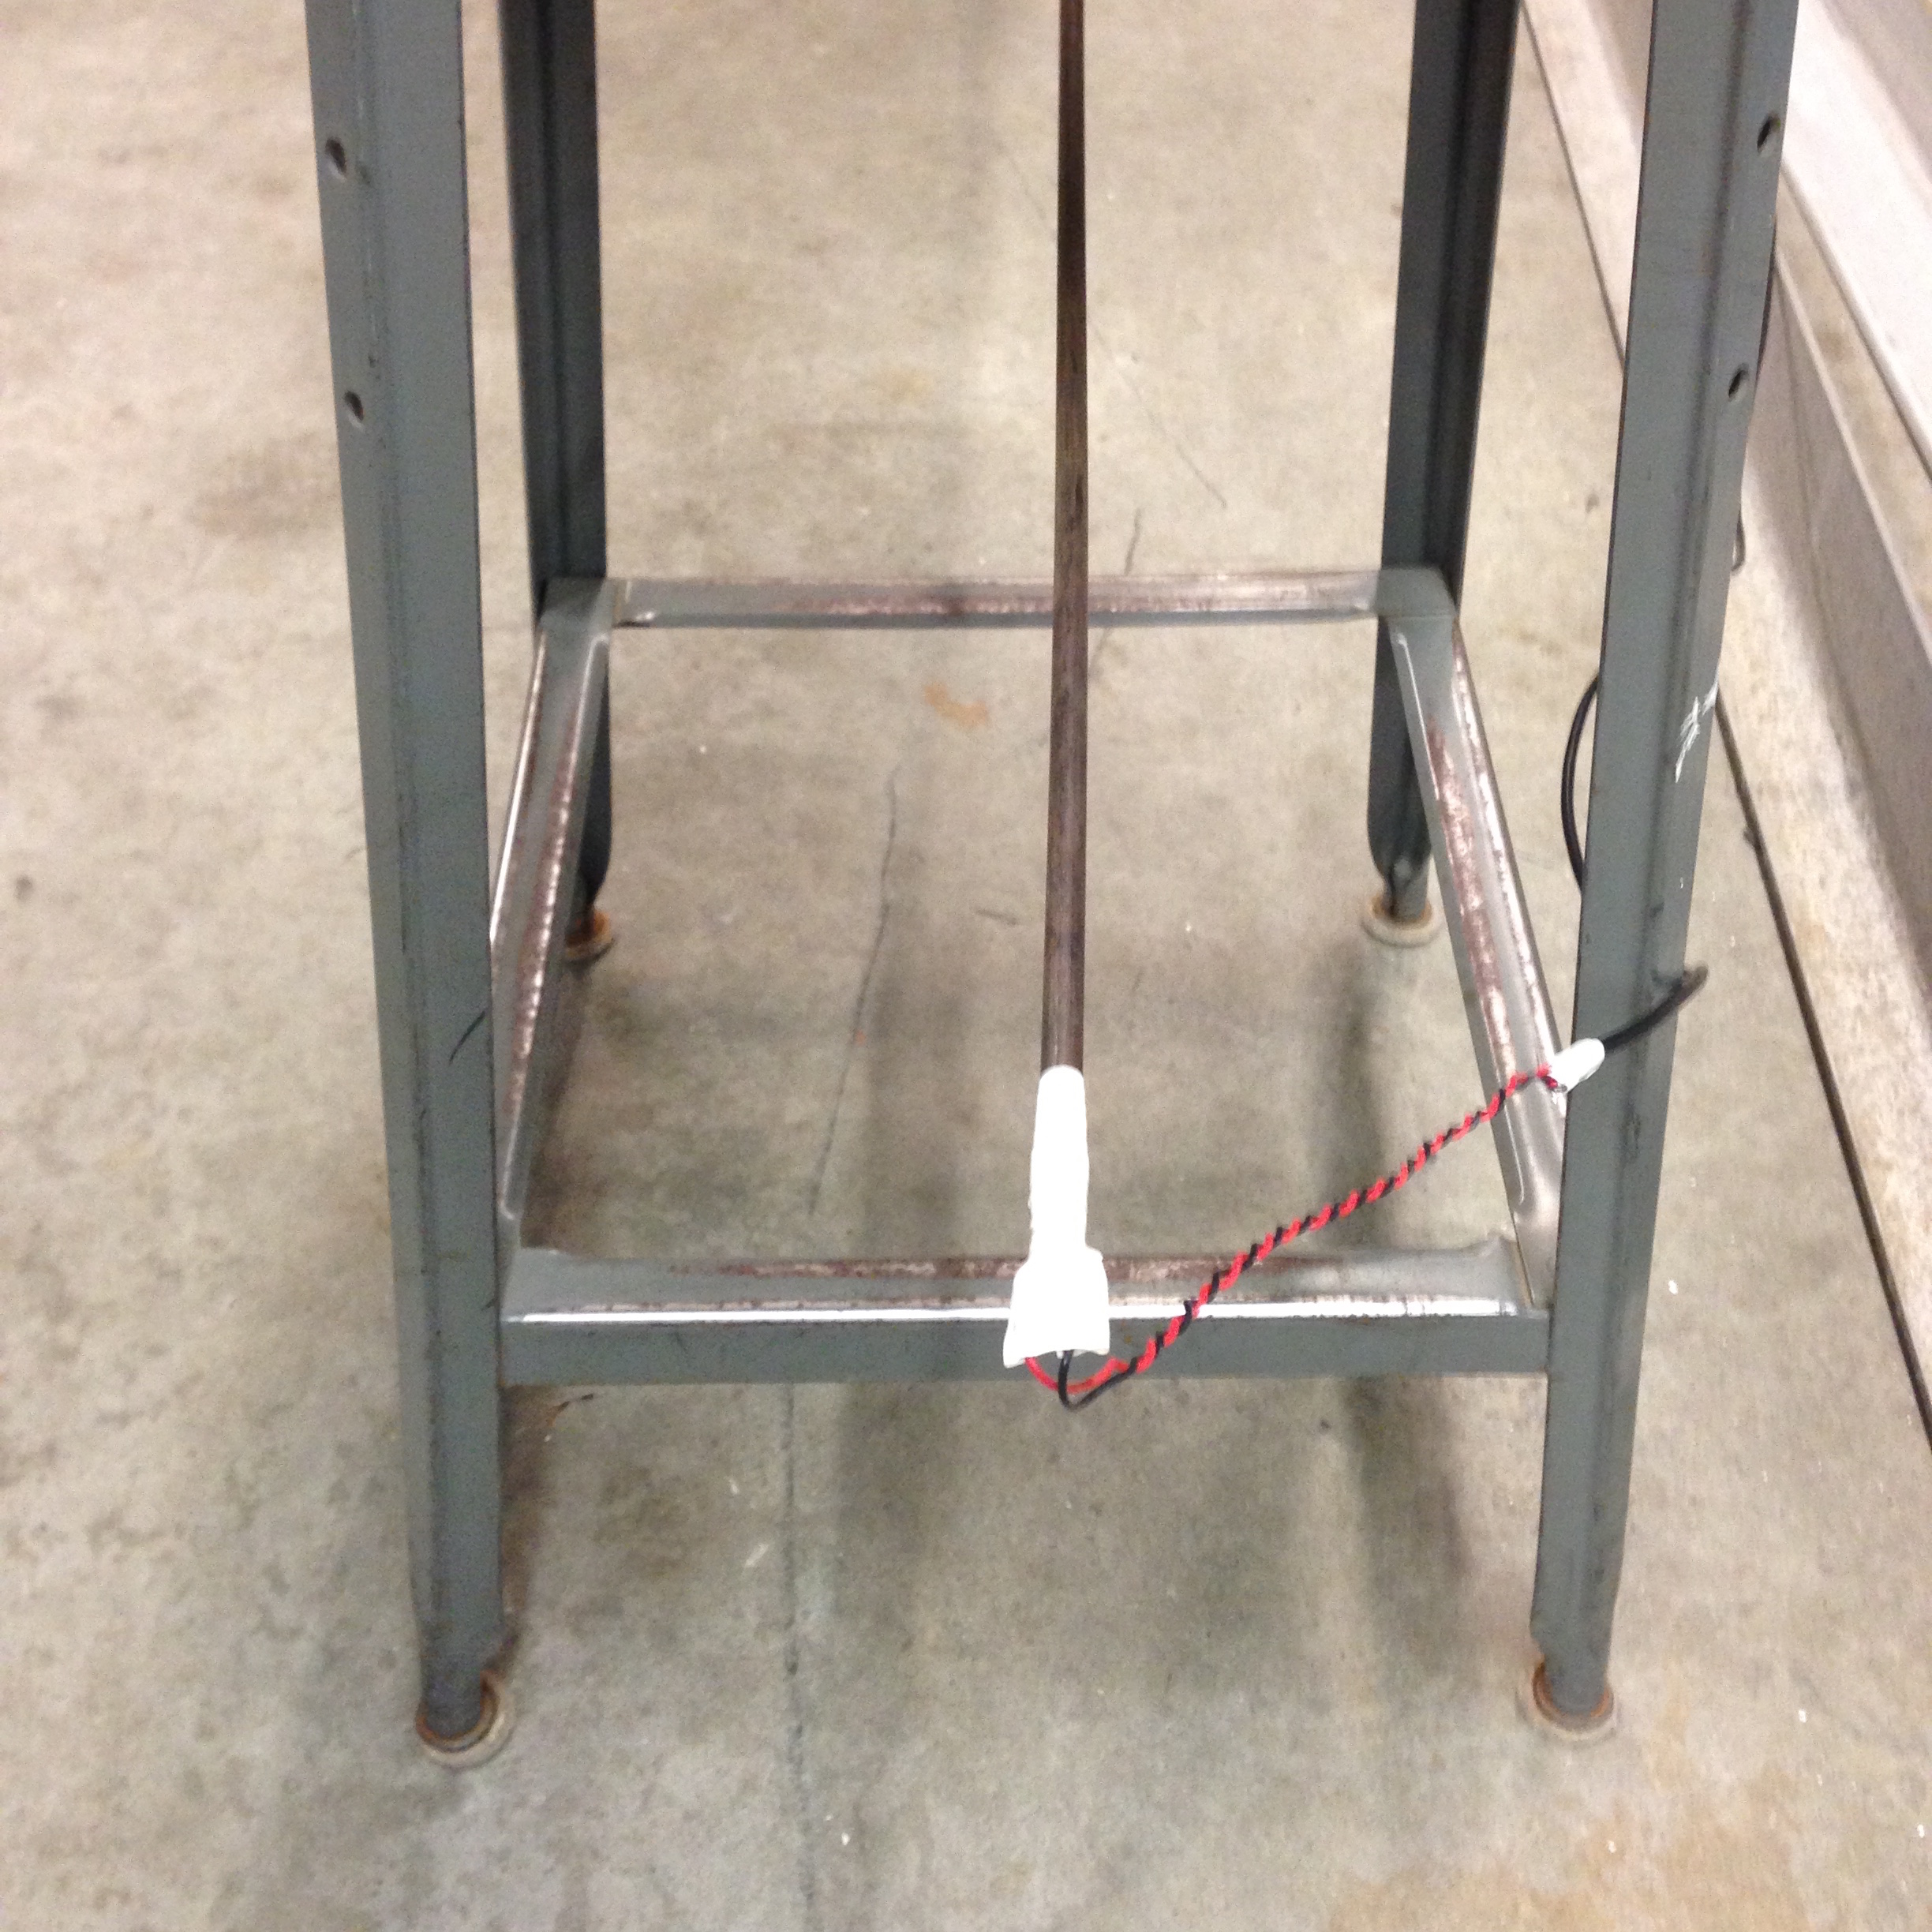
\includegraphics[width=.95\linewidth]{../figures/pmnt_end.jpg}
  \captionof{figure}{Another figure}
  \label{fig:rubbleband}
\end{minipage}
\end{figure}

The rod was excited mechanically using the strike of a hammer and a rubber mallet. With the piezoelectric sensor secured around the end of the rod as seen above, the rod was struck at the opposing endpoint using both the mallet and the hammer. This was done in order to produce an axial (or longitudinal) wave propagation down the length of the rod. The produced sound data was recorded in to individual files. The rod was then struck on its midpoint in the same manor in order to generate a transverse wave. The data was recorded for each striking surface. This procedure yielded 4 sets of sound data. The sets corresponded to metal and rubber strikes for both longitudinal and transverse excitations along the rod with the sensor recording near the endpoint. 

The sensor was then repositioned to the midpoint of the metal rod. Sound data was collected once again for transverse and longitudinal excitations. Once again the endpoint of the rod was struck longitudinally using both a hammer and rubber mallet to axially excite the rod. In order to excite the rod transversely, the rod was struck on its \emph{side} very close to the end point. These strikes were recorded individually to produce 4 more sets of data. This data corresponded to metal and rubber strikes for both longitudinal and transverse excitations along the rod with the sensor recording at the midpoint. 

\subsection{Results and Analysis}

The 8 data sets from the experiment were interpolated with MATLAB and cropped to the beginning of each strike. The cropped waveform for the axial rubber mallet strike, with the sensor recording from the opposite endpoint, can be seen below in Figure~\ref{fig:axial_endpoint}.

\begin{figure}[h]
	\centering
	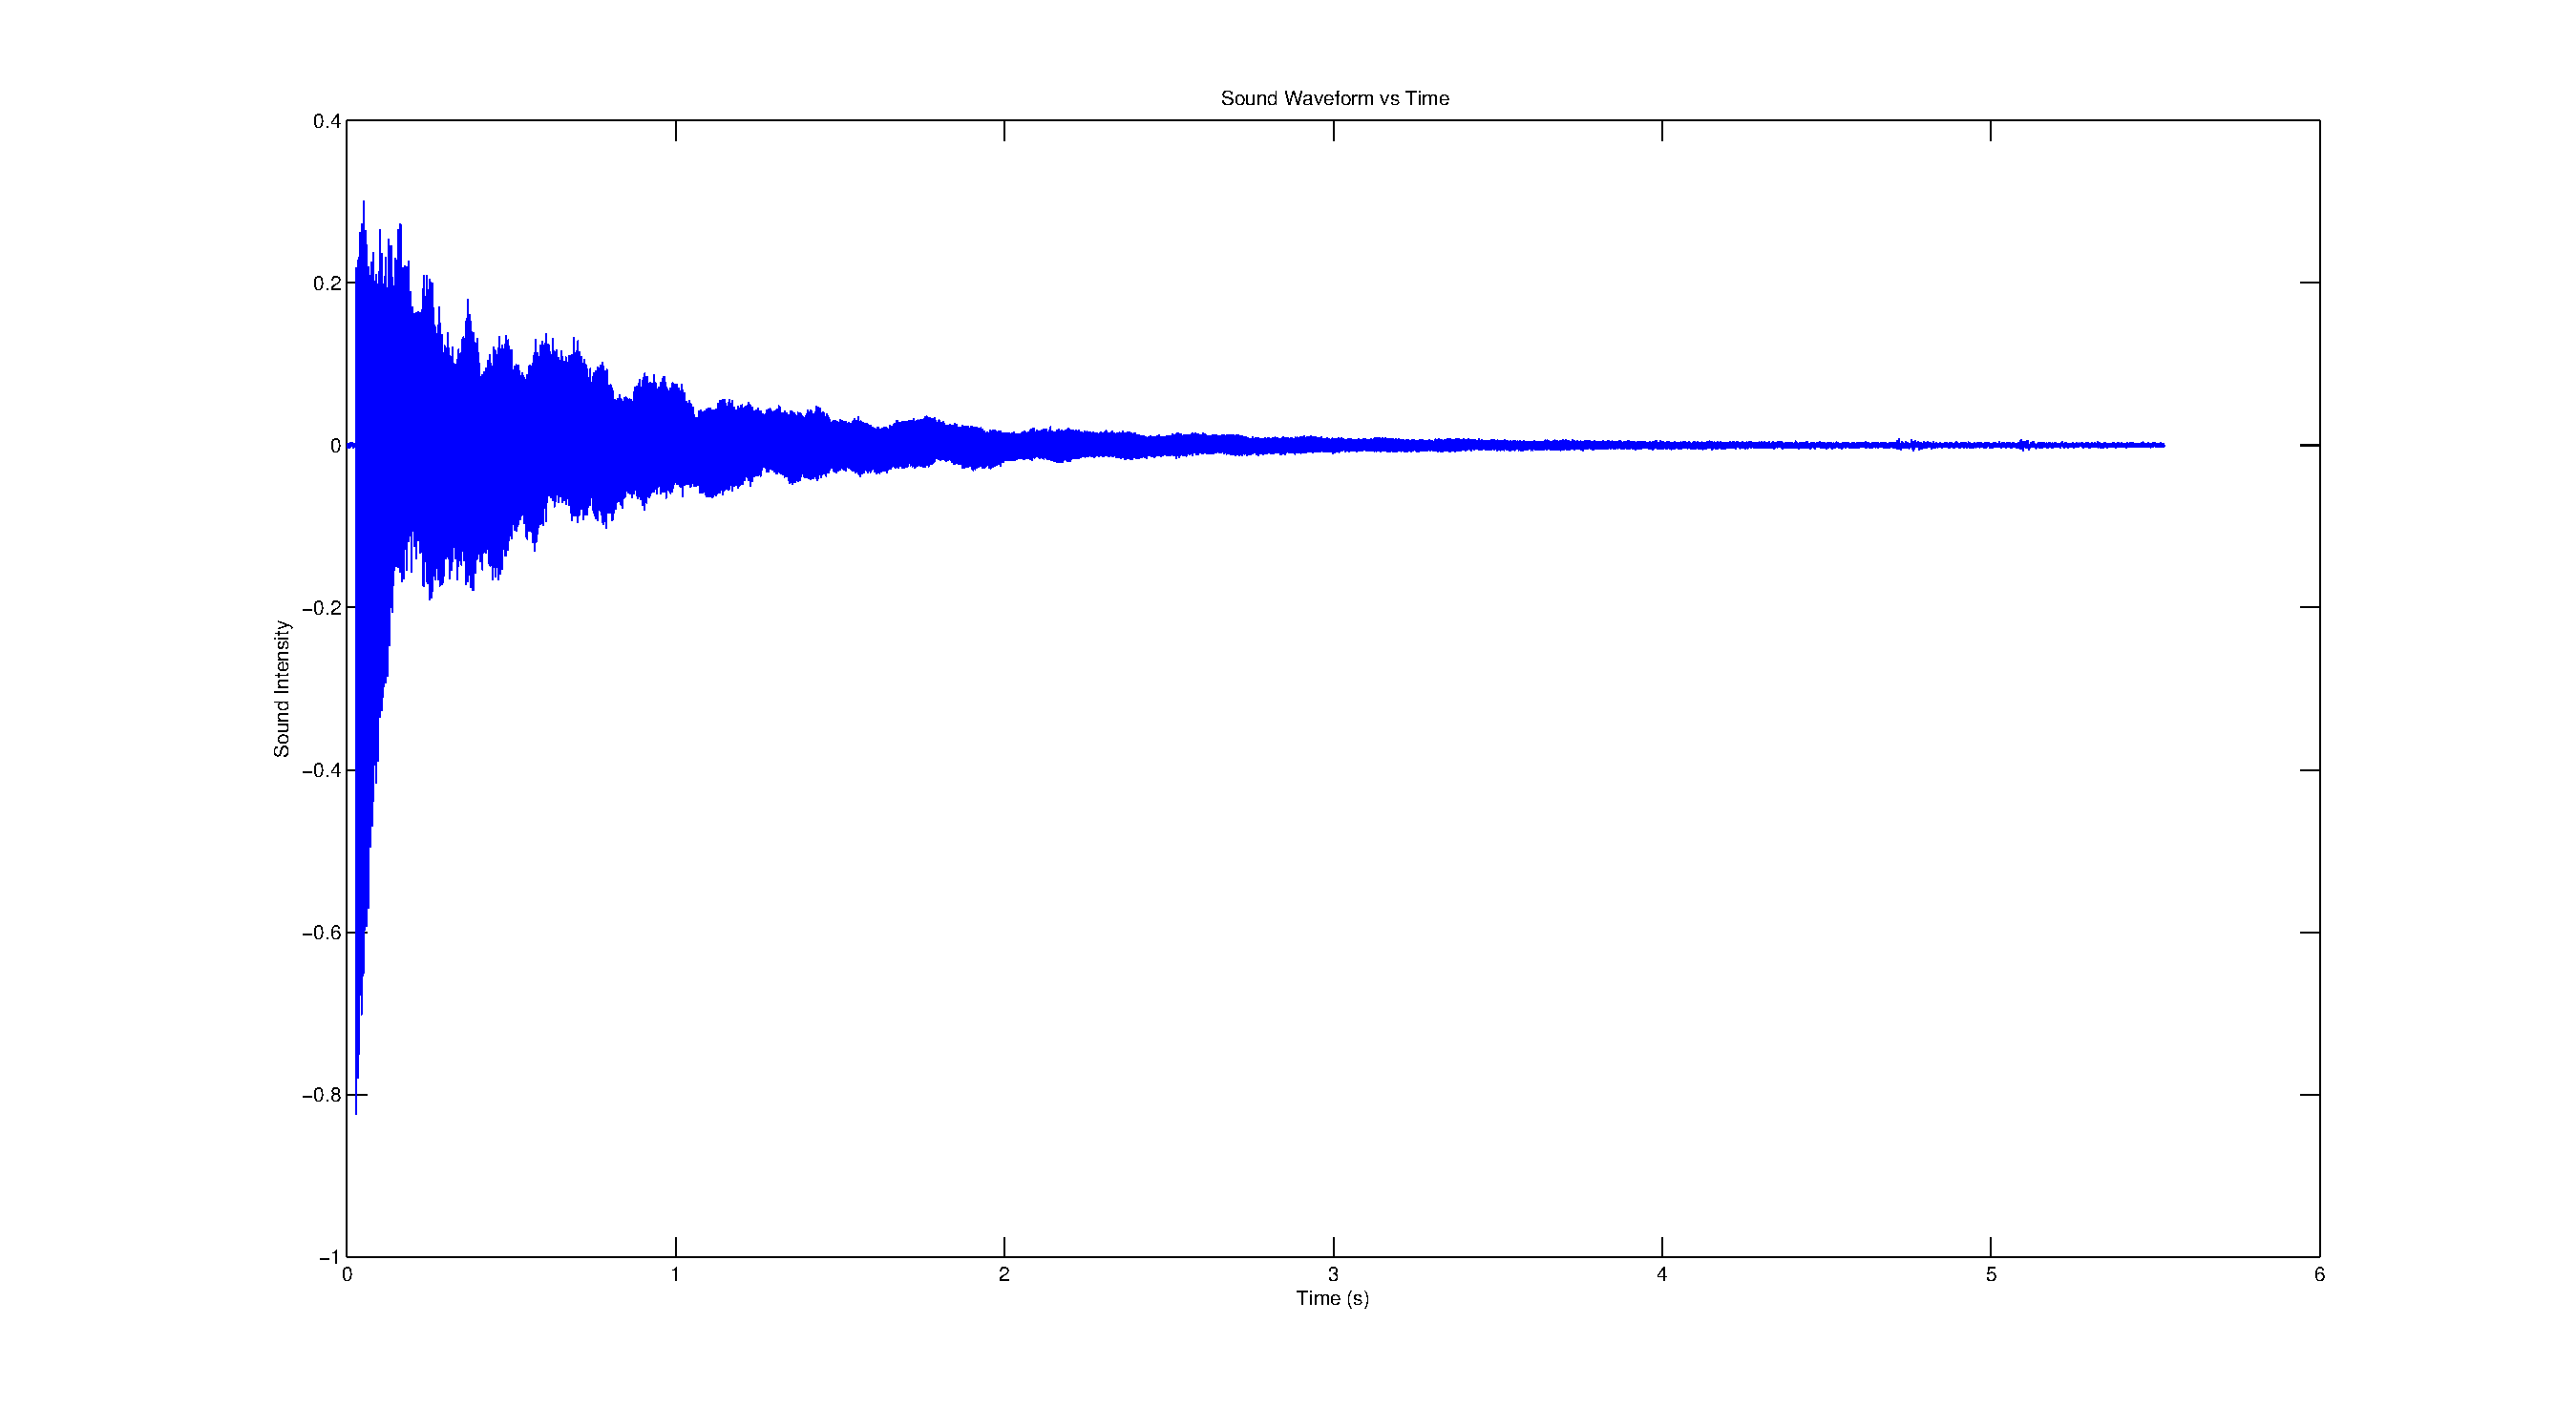
\includegraphics[width=\textwidth]{../figures/axial_rubber_endpoint.eps}
	\caption{Waveform for cropped rubber mallet axial strike (sensor at opposing endpoint)}
	\label{fig:axial_endpoint}
\end{figure}
	
This is an example of the sound data produced for each strike during the experimental trials. Each one of these datasets was then analyzed for frequency content using the two methods of Fourier Analysis and Prony's Method. The Fast Fourier Transform was taken for each dataset and the FFT of the above axial rubber strike can be seen below in Figure~\ref{fig:axial_FFT}.

\begin{figure}[h]
	\centering
	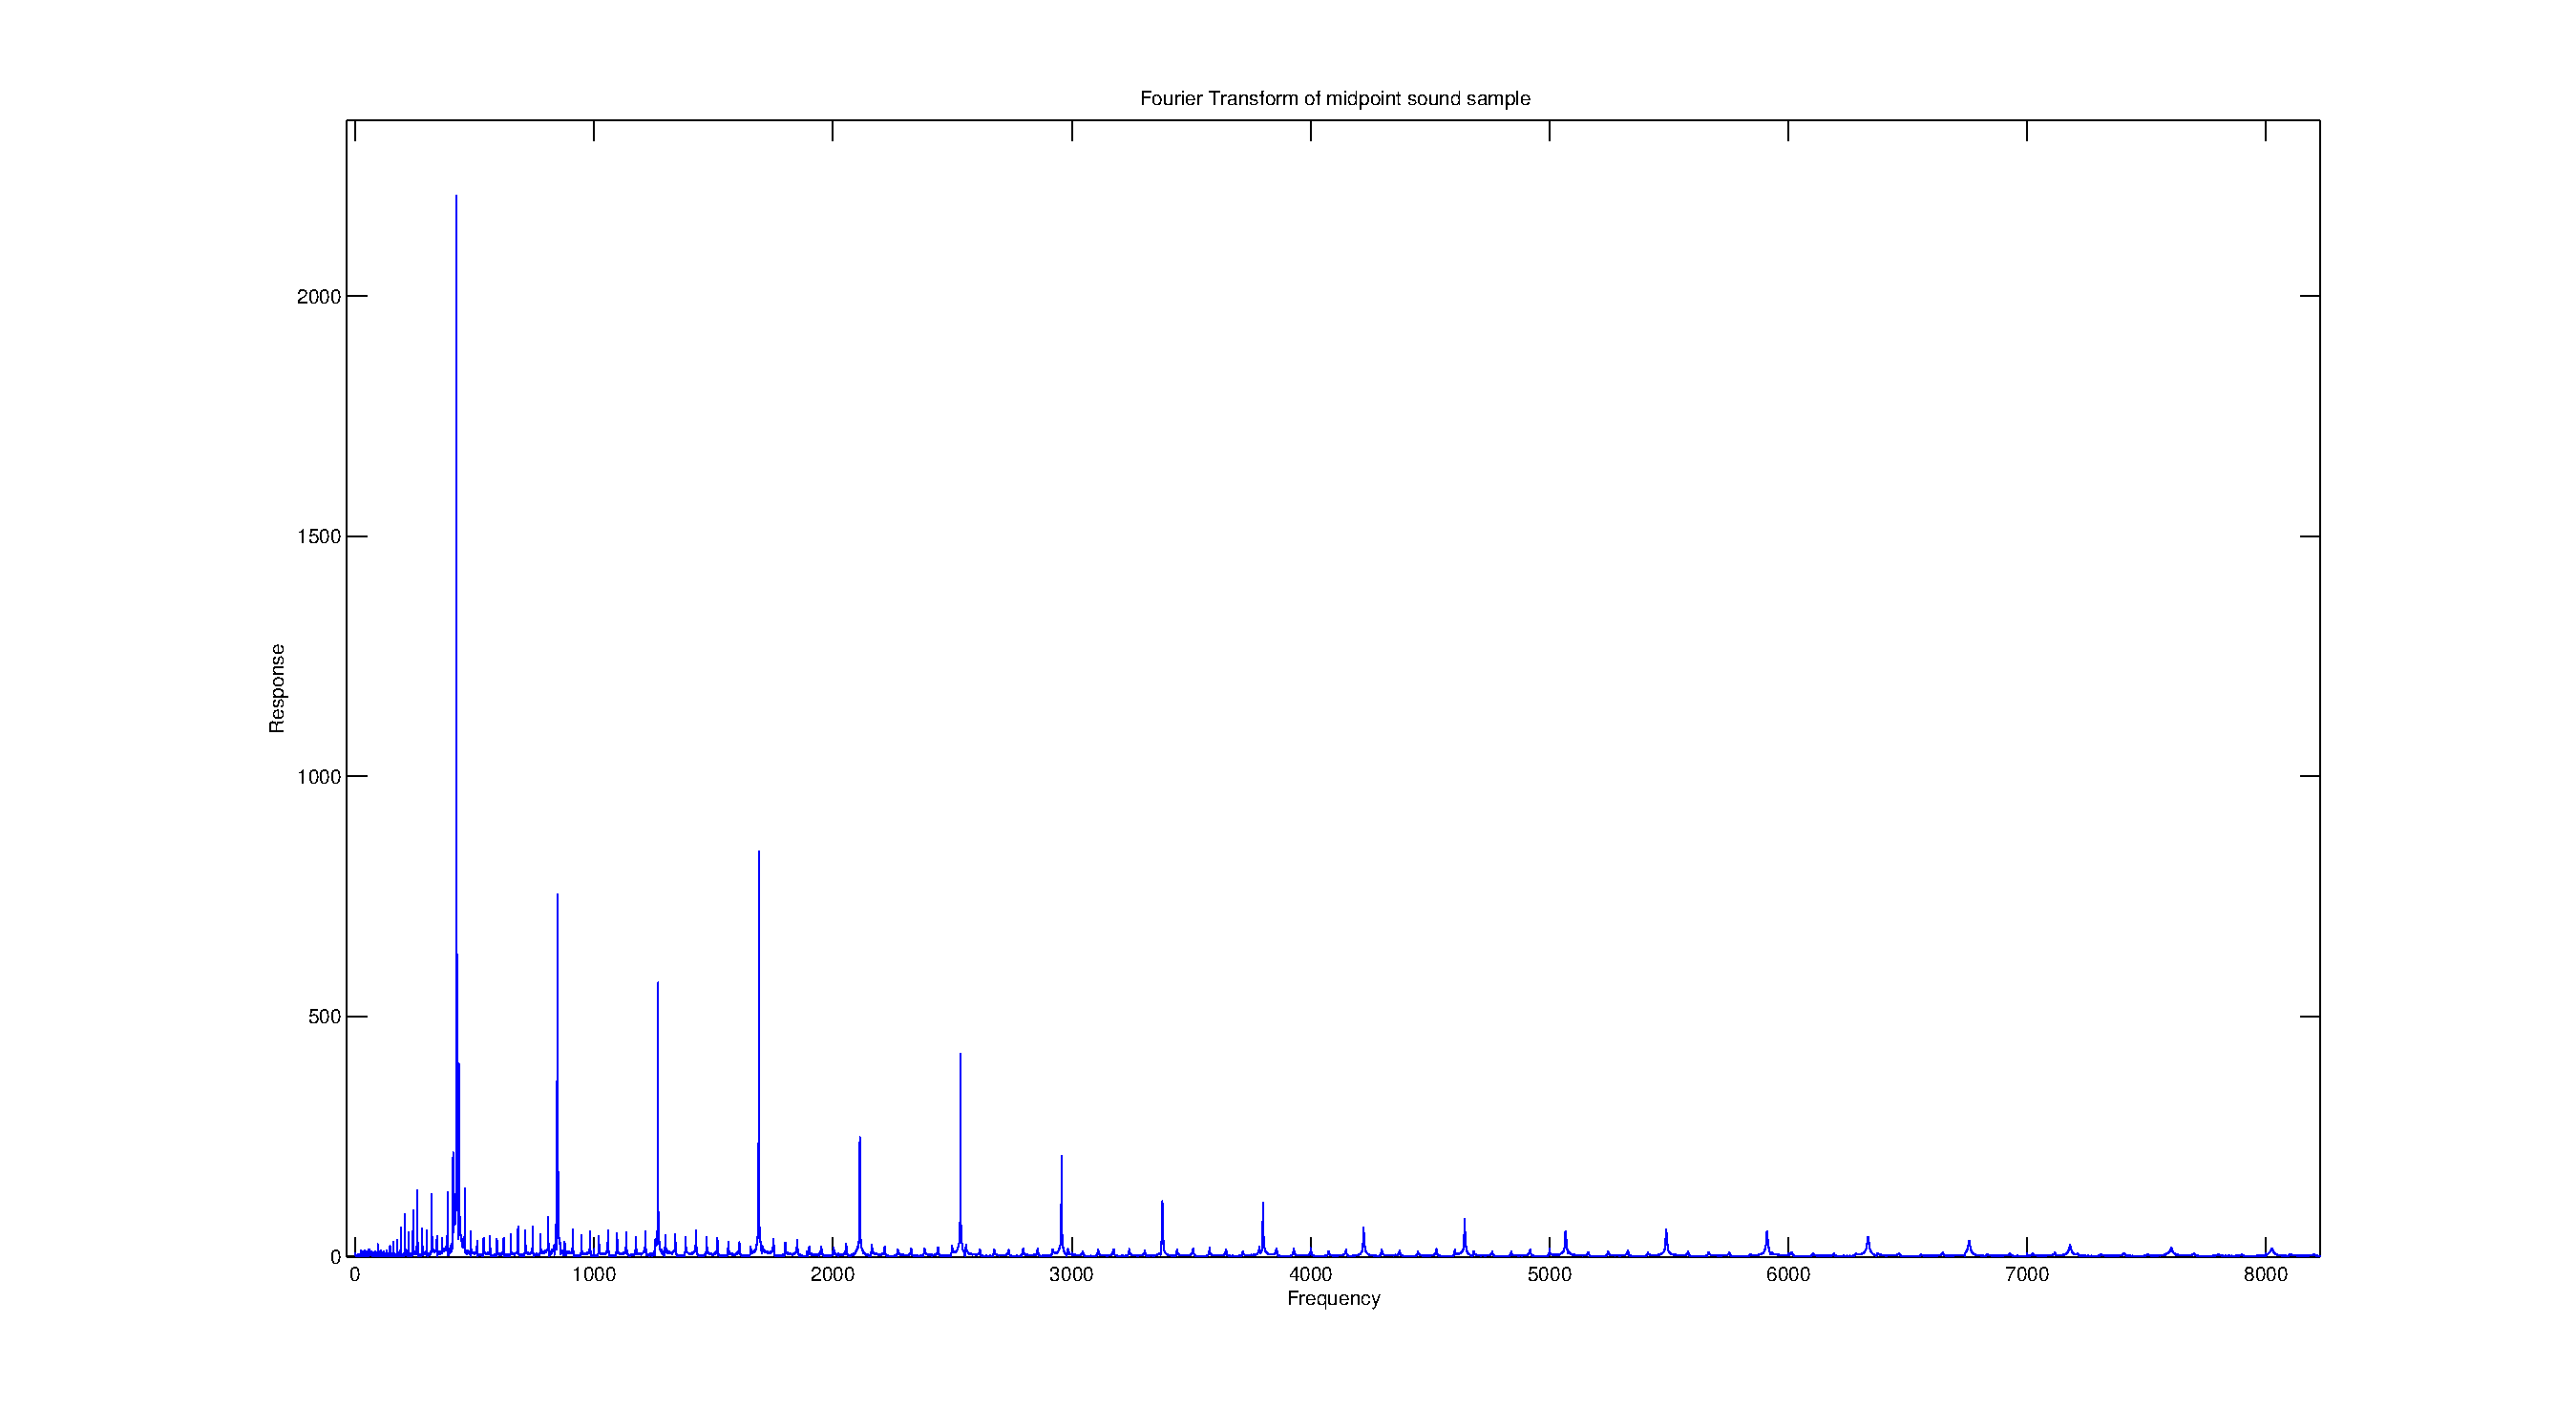
\includegraphics[width=\textwidth]{../figures/axial_rubber_endpointFFT.eps}
	\caption{FFT for cropped rubber mallet axial strike (sensor at opposing endpoint)}
	\label{fig:axial_FFT}
\end{figure}

Several definitive peaks can be seen steadily decreasing along the spectrum as frequency increases. These peaks correspond to the first several resonant modal frequencies of the free hanging rod in excitation. The first and strongest frequency response is seen to be at 424.8 Hz. This was repeated for each trial and the results were tabulated. It was discovered during this analysis that several of the data sets were very noisy and it was nearly impossible to extract a pattern of frequencies. The trials which produced these results were both the transverse excitations with the sensor near the endpoint and the transverse excitation using the rubber mallet with the sensor at the midpoint. An FFT from one of these noisy data sets can be seen below in Figure~\ref{fig:badFFT}.

\begin{figure}[h]
	\centering
	\includegraphics[width=\textwidth]{../figures/badFFT.eps}
	\caption{Noisy FFT data from transverse rubber mallet strike recorded at midpoint}
	\label{fig:badFFT}
\end{figure}


Prony analysis was also completed in order to determine the first strongest 8 frequencies present in the data for each trial. In the following tables, the results for both the Prony and Fourier Analysis can be seen alongside the expected theoretical frequencies calculated in the previous section. 



